\documentclass[../main.tex]{subfiles}
\begin{document}
\chapter{2015-2016学年微积分（一）（下）期末考试}

\section{单项选择题(每小题 3 分，共 18 分)}
\begin{enumerate}
  \item 曲面$z=4-x^{2}-y^{2}$上点$P$处的切平面平行于平面$2x+2y+z=1$，则点$P$的坐标是（\qquad）.

        \begin{tasks}[label=\textbf{\Alph*.}, label-width=1.5em, column-sep=1em](2)
          \task $(1,-1,2)$
          \task $(-1,1,2)$
          \task $(1,1,2)$
          \task $(-1,1,1)$
        \end{tasks}

  \item 考虑二元函数$f(x,y)$在点$(x_{0},y_{0})$处的以下 4 条性质：

        （1）两个偏导数存在；（2）两个偏导函数连续；（3）可微；（4）沿任意方向的方向导数存在.

        若用“$P\Rightarrow Q$”表示可由性质$P$推出性质$Q$，则有（\qquad）.

        \begin{tasks}[label=\textbf{\Alph*.}, label-width=1.5em, column-sep=1em](2)
          \task $(2)\Rightarrow(3)\Rightarrow(1)$
          \task $(3)\Rightarrow(2)\Rightarrow(1)$
          \task $(3)\Rightarrow(4)\Rightarrow(1)$
          \task $(3)\Rightarrow(1)\Rightarrow(4)$
        \end{tasks}

  \item 将二次积分$I=\int_{0}^{\frac{\pi}{4}}\,\mathrm{d}\theta\int_{0}^{1}f(r\cos\theta,r\sin\theta)r\,\mathrm{d}r$
        化为直角坐标系下的二次积分，正确的结果是（\qquad）.

        \begin{tasks}[label=\textbf{\Alph*.}, label-width=1.5em, column-sep=1em](2)
          \task $\displaystyle I=\int_{0}^{1}\,\mathrm{d}y\int_{y}^{\sqrt{1-y^{2}}}f(x,y)\,\mathrm{d}x$
          \task $\displaystyle I=\int_{0}^{1}\,\mathrm{d}x\int_{\sqrt{1-x^{2}}}^{x}f(x,y)\,\mathrm{d}y$
          \task $\displaystyle I=\int_{0}^{\frac{\sqrt2}{2}}\,\mathrm{d}y\int_{y}^{\sqrt{1-y^{2}}}f(x,y)\,\mathrm{d}x$
          \task $\displaystyle I=\int_{0}^{\frac{\sqrt2}{2}}\,\mathrm{d}x\int_{\sqrt{1-x^{2}}}^{x}f(x,y)\,\mathrm{d}y$
        \end{tasks}

  \item 设$S$是圆柱面$x^{2}+y^{2}=R^{2}(R>0)$被平面$z=0,z=h$截下的部分，则$\iint\limits_{S}(x^{2}+y^{2})\,\mathrm{d}S=\text{（\qquad）}.$

        \begin{tasks}[label=\textbf{\Alph*.}, label-width=1.5em, column-sep=1em](4)
          \task $-2\pi hR^{3}$
          \task $2\pi hR^{3}$
          \task $\pi hR^{3}$
          \task $\dfrac{\pi}{2}R^{4}h$
        \end{tasks}

  \item 下列命题中正确的是（\qquad）.

        \begin{tasks}[label=\textbf{\Alph*.}, label-width=1.5em, column-sep=1em](1)
          \task 若$\lim\limits_{n\to\infty}a_{n}=0$，则$\sum\limits_{n=1}^{\infty}a_{n}$收敛
          \task 若正项级数$\sum\limits_{n=1}^{\infty}a_{n}$收敛，且$l=\lim\limits_{n\to\infty}\dfrac{a_{n+1}}{a_{n}}$存在，则$l<1$
          \task 若$\lim\limits_{n\to\infty}\dfrac{a_{n}}{b_{n}}=1$且$\sum\limits_{n=1}^{\infty}b_{n}$收敛，则$\sum\limits_{n=1}^{\infty}a_{n}$收敛
          \task 若$\sum\limits_{n=1}^{\infty}a_{n}$绝对收敛，则$\sum\limits_{n=1}^{\infty}a_{2n}$绝对收敛
        \end{tasks}

  \item 设$f(x)=x+1(0\leq x\leq \pi)$，而$S(x)=\frac{a_{0}}{2}+\sum_{n=1}^{\infty}a_{n}\cos nx,\ -\infty<x<+\infty$，其中
        \[
          a_{n}=\frac{2}{\pi}\int_{0}^{\pi}f(x)\cos nx\,\mathrm{d}x,
        \]
        则$S\left(-\frac{\pi}{2}\right)=\text{（\qquad）}$.

        \begin{tasks}[label=\textbf{\Alph*.}, label-width=1.5em, column-sep=1em](4)
          \task $-\dfrac{\pi}{2}+1$
          \task $\dfrac{\pi}{2}+1$
          \task $-\dfrac{\pi}{2}-1$
          \task $\dfrac{\pi}{2}-1$
        \end{tasks}

\end{enumerate}

\section{填空题(每小题 4 分，共 16 分)}
\begin{enumerate}
  \setcounter{enumi}{6}
  \item 以曲线$
          \begin{cases}
            2x^{2}+y^{2}+z^{2}=16, \\
            x^{2}+y^{2}-z^{2}=0
          \end{cases}
        $
        为准线，母线平行于$x$轴的柱面方程是\underline{\hspace{3cm}}.

  \item 设$\boldsymbol{F}=(y,z,xy)$，$\boldsymbol{G}=(1,0,x)$，则$\mathbf{rot}(\boldsymbol{F}\times \boldsymbol{G})=$\underline{\hspace{3cm}}.

  \item 设$D:x^{2}+y^{2}\leq a^{2}(a>0)$，若
        $
          \iint\limits_{D}\sqrt{a^{2}-x^{2}-y^{2}}\,\mathrm{d}x\,\mathrm{d}y=\pi
        $，
        则$a=$\underline{\hspace{3cm}}.

  \item 设$L$为从$A(1,0)$到$B(2,1)$的曲线弧，则$
          \int_{L}\left(2xy-y^{4}+3\right)\,\mathrm{d}x+\left(x^{2}-4xy^{3}\right)\,\mathrm{d}y=
        $
        \underline{\hspace{3cm}}.

\end{enumerate}

\section{基本计算题(每小题 7 分，共 42 分)}
\begin{enumerate}
  \setcounter{enumi}{10}
  \item 求过点$P(1,2,3)$且与$z$轴相交、与平面$x+y+z-2=0$平行的直线方程.
        \vspace{10em}

  \item 设$z=f\left(\sin x,\dfrac{x}{y}\right)$，其中$f$具有二阶连续导数，求$\dfrac{\partial^{2}z}{\partial x\partial y}$.
        \vspace{10em}

  \item 设函数$y=y(x),z=z(x)$由方程$z=xf(x+y)$以及$F(x,y,z)=0$所确定，其中$f$具有一阶连续导数，$F$具有一阶连续偏导数，求$\dfrac{\mathrm{d}z}{\mathrm{d}x}$.
        \vspace{8em}

  \item 求三重积分$I=\iiint\limits_{V}(x^{2}+yz+z^{2})\,\mathrm{d}v$，其中$V:x^{2}+y^{2}+z^{2}\leq1$.
        \vspace{8em}

  \item 求曲线积分$I=\oint_{L}\left(x^{2}-y^{2}\right)\,\mathrm{d}x+\left(x^{2}+y^{2}\right)\,\mathrm{d}y$，其中$L$是圆周$x^{2}+y^{2}=x+y+1$，取正向.
        \vspace{8em}

  \item 求幂级数$\displaystyle\sum_{n=1}^{\infty}\dfrac{(x-3)^{n}}{n\cdot3^{n}}$的收敛域与和函数$S(x)$.
        \vspace{9em}
\end{enumerate}

\section{应用题(每小题 7 分，共 14 分)}
\begin{enumerate}
  \setcounter{enumi}{16}
  \item 在椭球面$x^{2}+2y^{2}+2z^{2}=1$上求一点，使函数$f(x,y,z)=x^{2}+y^{2}+z^{2}$在该点处沿方向$\boldsymbol{n}=(0,-1,1)$的方向导数最大.
        \vspace{9em}

  \item 设速度场$\boldsymbol{v}=\left(2x^{3},2y^{3},3(z^{2}-1)\right)$，$S$是曲面$z=1-x^{2}-y^{2}(z\geq0)$的上侧，求单位时间内流过曲面$S$上侧的通量
        \[
          \varPhi=\iint\limits_{S}\boldsymbol{v}\cdot\boldsymbol{n}\,\mathrm{d}S.
        \]
        \vspace{13em}
\end{enumerate}

\section{综合题(每小题 5 分，共 10 分)}
\begin{enumerate}
  \setcounter{enumi}{18}
  \item 证明Leibniz判别法：若数项级数$\displaystyle\sum_{n=1}^{\infty}(-1)^{n-1}a_{n}(a_{n}>0)$满足（1）$\lim\limits_{n\to\infty}a_{n}=0$；（2）$\{a_{n}\}$单调减少，则级数$\displaystyle\sum_{n=1}^{\infty}(-1)^{n-1}a_{n}$收敛.
        \vspace{13em}

  \item 设函数$f(x,y)$具有二阶连续偏导数，且$f(1,y)=0,f(x,1)=0,\iint\limits_{D}f(x,y)\,\mathrm{d}\sigma=a$，其中$D:0\leq x\leq1,0\leq y\leq1$。计算积分
        \[
          I=\iint\limits_{D}xyf_{xy}(x,y)\,\mathrm{d}\sigma.
        \]
        \vspace{13em}
\end{enumerate}

\chapter{2015-2016学年微积分（一）（下）期末考试参考答案}
\section{单项选择题(每小题 3 分，共 18 分)}
\begin{enumerate}
  \item \textbf{Solution}. C.

        曲面可写成$F(x,y,z)=x^2+y^2+z-4=0$，其法向量为
        \[
          \nabla F=(2x,2y,1).
        \]
        切平面平行于平面$2x+2y+z=1$，故两平面的法向量平行，即
        \[
          \frac{2x}{2}=\frac{2y}{2}=\frac{1}{1},
        \]
        解得$x=1,y=1$. 代入曲面方程得$z=2$，故$P=(1,1,2)$.

  \item \textbf{Solution}. A.

        两个偏导函数在点$(x_0,y_0)$处连续可推出函数在该点可微；可微又必推出两个偏导数存在.

        但偏导数存在不能推出可微；可微也不能推出偏导函数连续. 因此成立的是
        \[
          (2)\Rightarrow(3)\Rightarrow(1).
        \]

  \item \textbf{Solution}. C.

        \noindent
        \begin{minipage}[c]{0.65\textwidth}
          原积分区域在极坐标下为
          \[
            0\leq r\leq1,\qquad 0\leq \theta\leq\frac{\pi}{4},
          \]
          即第一象限中由$x$轴、直线$y=x$和圆$x^2+y^2=1$围成的扇形区域.

          改用直角坐标时，$0\le y\le \dfrac{\sqrt2}{2}$，且对固定的$y$，有
          \[
            y\le x\le \sqrt{1-y^2}.
          \]
        \end{minipage}
        \hfill %
        \begin{minipage}[c]{0.4\textwidth}
          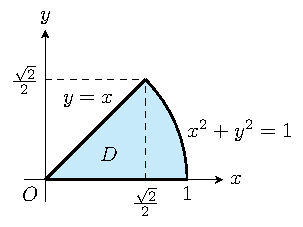
\includegraphics[width=5cm]{2016xf-figure1.pdf}
        \end{minipage}

        因而
        \[
          I=\int_{0}^{\frac{\sqrt2}{2}}\,\mathrm{d}y\int_{y}^{\sqrt{1-y^{2}}}f(x,y)\,\mathrm{d}x.
        \]

  \item \textbf{Solution}. B.

        在圆柱面上$x^2+y^2=R^2$，故被积函数恒为$R^2$. 圆柱侧面积为$2\pi Rh$，所以
        \[
          \iint\limits_S(x^2+y^2)\,\mathrm{d}S=R^2\cdot2\pi Rh=2\pi hR^3.
        \]

  \item \textbf{Solution}. D.

        对于A选项，令$a_n=\dfrac1n$，则$\lim\limits_{n\to\infty}a_n=0$，但调和级数$\sum_{n=1}^{\infty}\frac1n$发散.

        对于B选项，令$a_n=\dfrac1{n^2}$，则$\sum\limits_{n=1}^{\infty}a_n$收敛，但$
          l=\lim_{n\to\infty}\frac{a_{n+1}}{a_n}
          =\lim_{n\to\infty}\frac{n^2}{(n+1)^2}=1$.

        对于C选项，令
        \[
          a_n=\frac{(-1)^n}{\sqrt n}+\frac1n,\qquad
          b_n=\frac{(-1)^n}{\sqrt n},
        \]
        则$\sum b_n$由Leibniz判别法可知收敛，且
        \[
          \lim_{n\to\infty}\frac{a_n}{b_n}
          =\lim_{n\to\infty}\left(1+\frac{\frac{1}{n}}{\frac{(-1)^n}{\sqrt n}}\right)
          =\lim_{n\to\infty}\left(1+\frac{(-1)^n}{\sqrt n}\right)=1.
        \]
        但$\sum a_n=\sum b_n+\sum\dfrac1n$发散.

        对于D选项，若$\sum a_n$绝对收敛，则$\sum |a_n|$收敛. 又$\sum |a_{2n}|$是$\sum |a_n|$的子级数，故$\sum |a_{2n}|$收敛，

        因而$\sum a_{2n}$绝对收敛，故D正确.

  \item \textbf{Solution}. B.

        该级数是$f(x)=x+1\ (0\le x\le\pi)$作偶延拓后的余弦级数，因此其和函数为周期为$2\pi$的偶函数.

        故
        \[
          S\left(-\frac{\pi}{2}\right)=S\left(\frac{\pi}{2}\right)
          =f\left(\frac{\pi}{2}\right)=\frac{\pi}{2}+1.
        \]
\end{enumerate}

\section{填空题(每小题 4 分，共 16 分)}
\begin{enumerate}
  \setcounter{enumi}{6}
  \item \textbf{Solution}. $3z^{2}-y^{2}=16$.

        母线平行于$x$轴，故所求柱面方程中应消去$x$. 由
        \[
          x^2+y^2-z^2=0
        \]
        得$x^2=z^2-y^2$. 代入$2x^2+y^2+z^2=16$，得
        \[
          2(z^2-y^2)+y^2+z^2=16,
        \]
        即
        \[
          3z^2-y^2=16.
        \]

  \item \textbf{Solution}. $(0,x,0)$.

        先求
        \[
          \boldsymbol{F}\times\boldsymbol{G}
          =
          \begin{vmatrix}
            \boldsymbol{i} & \boldsymbol{j} & \boldsymbol{k} \\
            y              & z              & xy             \\
            1              & 0              & x
          \end{vmatrix}
          =(xz,0,-z).
        \]
        因此
        \[
          \mathbf{rot}(\boldsymbol{F}\times\boldsymbol{G})
          =
          \left(
          \frac{\partial(-z)}{\partial y}-\frac{\partial 0}{\partial z},
          \frac{\partial(xz)}{\partial z}-\frac{\partial(-z)}{\partial x},
          \frac{\partial 0}{\partial x}-\frac{\partial(xz)}{\partial y}
          \right)
          =(0,x,0).
        \]

  \item \textbf{Solution}. $\sqrt[3]{\dfrac{3}{2}}$.

        用极坐标代换，
        \[
          \iint\limits_D\sqrt{a^2-x^2-y^2}\,\mathrm{d}x\,\mathrm{d}y
          =2\pi\int_0^a r\sqrt{a^2-r^2}\,\mathrm{d}r
          =\frac{2\pi a^3}{3}.
        \]
        由题设得$\dfrac{2\pi a^3}{3}=\pi$，故
        \[
          a^3=\frac32,\qquad a=\sqrt[3]{\frac32}.
        \]

  \item \textbf{Solution}. $5$.

        记
        \[
          P=2xy-y^4+3,\qquad Q=x^2-4xy^3.
        \]
        因为$P_y=2x-4y^3=Q_x$，所以该曲线积分与路径无关.

        取势函数$\Phi$，由$\Phi_x=P$得
        \[
          \Phi=x^2y-xy^4+3x+\varphi(y).
        \]
        再由$\Phi_y=Q$可知$\varphi'(y)=0$，故可取$\Phi=x^2y-xy^4+3x$. 因而
        \[
          \int_LP\,\mathrm{d}x+Q\,\mathrm{d}y
          =\Phi(2,1)-\Phi(1,0)=6-1=5.
        \]
\end{enumerate}

\section{基本计算题(每小题 7 分，共 42 分)}
\begin{enumerate}
  \setcounter{enumi}{10}
  \item \textbf{Solution}. 设所求直线的方向向量为$\boldsymbol{s}$，并与$z$轴相交于点$Q(0,0,c)$，则
        \[
          \boldsymbol{s}=\overrightarrow{PQ}=(-1,-2,c-3).
        \]
        由题设知$\boldsymbol{s}\perp(1,1,1)$，故$c=6$.
        所求直线方程为
        \[
          \frac{x-1}{1}=\frac{y-2}{2}=\frac{z-3}{-3}.
        \]

  \item \textbf{Solution}. 记$f_{1},f_{2},f_{12},f_{22}$分别表示$f$对其变量的一阶、二阶偏导数，则
        \[
          \frac{\partial z}{\partial x}=\cos x\,f_{1}+\frac{1}{y}f_{2}.
        \]
        因而
        \[
          \frac{\partial^2 z}{\partial x \partial y}=-\frac{x\cos x}{y^{2}}f_{12}-\frac{1}{y^{2}}f_{2}-\frac{x}{y^{3}}f_{22}.
        \]

  \item \textbf{Solution}. 对方程组
        \[
          \begin{cases}
            z=xf(x+y), \\
            F(x,y,z)=0
          \end{cases}
        \]
        两边对$x$求导，得
        \[
          \begin{cases}
            \dfrac{\mathrm{d}z}{\mathrm{d}x}=f+x\left(1+\dfrac{\mathrm{d}y}{\mathrm{d}x}\right)f', \\[8pt]
            F_{1}+\dfrac{\mathrm{d}y}{\mathrm{d}x}F_{2}+\dfrac{\mathrm{d}z}{\mathrm{d}x}F_{3}=0.
          \end{cases}
        \]
        消去$\dfrac{\mathrm{d}y}{\mathrm{d}x}$可得
        \[
          \frac{\mathrm{d}z}{\mathrm{d}x}
          =\frac{(f+xf')F_{2}-xf'F_{1}}{F_{2}+xf'F_{3}}.
        \]

  \item \textbf{Solution}. 由球域的对称性可知
        \[
          \iiint\limits_{V}yz\,\mathrm{d}v=0,\qquad
          \iiint\limits_{V}(x^{2}+yz+z^{2})\,\mathrm{d}v
          =\frac{2}{3}\iiint\limits_{V}(x^{2}+y^{2}+z^{2})\,\mathrm{d}v.
        \]
        用球坐标代换，
        \[
          I=\frac{2}{3}\int_{0}^{2\pi}\,\mathrm{d}\theta\int_{0}^{\pi}\sin\varphi\,\mathrm{d}\varphi\int_{0}^{1}\rho^{4}\,\mathrm{d}\rho
          =\frac{8\pi}{15}.
        \]

  \item \textbf{Solution}. 由Green公式，
        \[
          I=\iint\limits_{D}\left[\frac{\partial(x^{2}+y^{2})}{\partial x}-\frac{\partial(x^{2}-y^{2})}{\partial y}\right]\mathrm{d}x\,\mathrm{d}y
          =\iint\limits_{D}2(x+y)\,\mathrm{d}x\,\mathrm{d}y.
        \]
        圆周$x^{2}+y^{2}=x+y+1$所围区域$D$的圆心为$\left(\dfrac12,\dfrac12\right)$，半径为$\sqrt{\dfrac32}$，
        故
        \[
          I=2(\bar{x}+\bar{y})\sigma=2\cdot1\cdot\frac{3\pi}{2}=3\pi.
        \]

  \item \textbf{Solution}. 记$a_n=\frac{1}{n3^n}$，用比值判别法计算
        \[
          \rho = \lim_{n \to \infty} \left| \frac{a_{n+1}}{a_n} \right| = \lim_{n \to \infty} \frac{n \cdot 3^n}{(n+1) \cdot 3^{n+1}} = \frac{1}{3} \lim_{n \to \infty} \frac{n}{n+1} = \frac{1}{3},
        \]
        从而收敛半径$R=\frac{1}{\rho}=3$.

        当$x=6$时，原级数化为调和级数$\sum_{n=1}^{\infty}\frac1n$，因而发散；

        当$x=0$时，原级数化为交错调和级数$\sum_{n=1}^{\infty}\frac{(-1)^n}{n}$，因而收敛.

        故原级数收敛域为$[0,6)$. 下面计算其和函数$S(x)=\sum_{n=1}^{\infty}\frac{(x-3)^n}{n\cdot3^n}$.

        对$S(x)$求导，得
        \[
          S'(x) = \sum_{n=1}^{\infty} \frac{n(x-3)^{n-1}}{n \cdot 3^n} = \sum_{n=1}^{\infty} \frac{(x-3)^{n-1}}{3^n}=\frac{1}{3}\sum_{n=0}^{\infty} \left(\frac{x-3}{3}\right)^n,
        \]

        这是一个首项为 $\frac{1}{3}$，公比为 $\frac{x-3}{3}$ 的几何级数，因此$S'(x) = \frac{\frac{1}{3}}{1 - \frac{x-3}{3}} = \frac{1}{3 - (x-3)} = \frac{1}{6-x}$.

        注意到$S(3) = 0$，因此
        \[
          S(x) = \int_{3}^{x} \frac{1}{6-t} \, dt = -\ln|6-x| + \ln|3| = \ln\left(\frac{3}{6-x}\right), \quad x \in [0, 6).
        \]

\end{enumerate}

\section{应用题(每小题 7 分，共 14 分)}
\begin{enumerate}
  \setcounter{enumi}{16}
  \item \textbf{Solution}. 设所求点为$M(x,y,z)$，则
        \[
          \nabla f(M)=(2x,2y,2z),\qquad \boldsymbol{n}^{\circ}=\frac{1}{\sqrt2}(0,-1,1).
        \]
        故方向导数为
        \[
          \frac{\partial f(M)}{\partial \boldsymbol{n}}=\sqrt2(-y+z).
        \]
        即在约束条件$x^{2}+2y^{2}+2z^{2}=1$下，求$-y+z$的最大值.

        用Lagrange乘数法，设$L(x,y,z,\lambda)=-y+z+\lambda(x^{2}+2y^{2}+2z^{2}-1)$，令$\nabla L=0$，得
        \[
          \begin{cases}
            2\lambda x=0,   \\
            4\lambda y-1=0, \\
            4\lambda z+1=0, \\
            x^{2}+2y^{2}+2z^{2}=1.
          \end{cases}
        \]

        由前两个方程可知$x=0$，且$z=-y$. 代入约束方程得
        \[
          4y^{2}=1,\qquad y=\pm\frac12,\qquad z=\mp\frac12.
        \]
        因而受检点为
        \[
          M_1\left(0,\frac12,-\frac12\right),\qquad M_2\left(0,-\frac12,\frac12\right).
        \]
        比较方向导数的值，
        \[
          \frac{\partial f(M_1)}{\partial \boldsymbol{n}}=-\sqrt2,\qquad
          \frac{\partial f(M_2)}{\partial \boldsymbol{n}}=\sqrt2,
        \]
        故所求点为
        \[
          \left(0,-\frac12,\frac12\right).
        \]

  \item \textbf{Solution}. 取底面$S_{1}:z=0,\ x^{2}+y^{2}\leq1$的下侧，使$S+S_{1}$封闭并取外侧法向.

        由Gauss公式，
        \[
          \begin{aligned}
            \varPhi={} & \oiint\limits_{S+S_{1}}\left(2x^3,2y^3,2z^3\right)\cdot\boldsymbol{n}\,\mathrm{d}S-\iint\limits_{S_{1}}3(z^{2}-1)\,\mathrm{d}x\,\mathrm{d}y \\
            ={}        & \iiint\limits_{V}\left(6x^2+6y^2+6z\right)\,\mathrm{d}v+3\iint\limits_{S_{1}}\,\mathrm{d}x\,\mathrm{d}y.
          \end{aligned}
        \]
        用柱坐标代换，
        \[
          \begin{aligned}
            \varPhi= {} & 6\iiint\limits_{V}\left(x^2+y^2+z\right)\,\mathrm{d}v+3\iint\limits_{S_{1}}\,\mathrm{d}x\,\mathrm{d}y                                                                       \\
            = {}        & 6\int_{0}^{1}\,\mathrm{d}z\int_{0}^{2\pi}\,\mathrm{d}\theta\int_{0}^{\sqrt{1-z}}r\left(r^2+z\right)\,\mathrm{d}r-3\iint\limits_{x^{2}+y^{2}\leq1}\,\mathrm{d}x\,\mathrm{d}y \\
            = {}        & 12\pi\int_{0}^{1}\left[\frac{1}{4}(1-z)^2+\frac{1}{2}(1-z)z\right]\,\mathrm{d}z-3\pi                                                                                        \\
            = {}        & 3\pi\int_{0}^{1}\left(1-z^2\right)\,\mathrm{d}z-3\pi=-\pi.
          \end{aligned}
        \]

\end{enumerate}

\section{综合题(每小题 5 分，共 10 分)}
\begin{enumerate}
  \setcounter{enumi}{18}
  \item \textbf{Proof}. 记部分和
        \[
          S_n=a_1-a_2+a_3-a_4+\cdots+(-1)^{n-1}a_n.
        \]
        对偶数项部分和，有
        \[
          S_{2n}=(a_1-a_2)+(a_3-a_4)+\cdots+(a_{2n-1}-a_{2n}).
        \]
        由于$\{a_n\}$单调减少，故$a_{2k-1}-a_{2k}\geq0$，从而$\{S_{2n}\}$单调增加.

        又
        \[
          S_{2n}=a_1-(a_2-a_3)-\cdots-(a_{2n-2}-a_{2n-1})-a_{2n}\leq a_1,
        \]
        因而$\{S_{2n}\}$单调有界，故收敛. 设
        \[
          \lim_{n\to\infty}S_{2n}=S.
        \]

        对奇数项部分和，
        \[
          S_{2n+1}=S_{2n}+a_{2n+1}.
        \]
        由$\lim\limits_{n\to\infty}a_n=0$可得
        \[
          \lim_{n\to\infty}S_{2n+1}=S.
        \]
        因此奇、偶部分和有相同极限$S$，故原级数收敛.

  \item \textbf{Solution}. 因$f(1,y)=0,f(x,1)=0$，所以
        \[
          f_{y}(1,y)=0,\qquad f_{x}(x,1)=0.
        \]
        由两次分部积分，
        \[
          \begin{aligned}
            I= {} & \iint\limits_{D}xyf_{xy}(x,y)\,\mathrm{d}\sigma=\int_{0}^{1}\,\mathrm{d}x\int_{0}^{1}xyf_{xy}(x,y)\,\mathrm{d}y                                                                       \\
            = {}  & \int_{0}^{1}\left[\int_{0}^{1}xy\,\mathrm{d}f_{x}(x,y)\right]\,\mathrm{d}x = \int_{0}^{1}\left[xyf_{x}(x,y)\Big|_{y=0}^{y=1}-\int_{0}^{1}xf_{x}(x,y)\,\mathrm{d}y\right]\,\mathrm{d}x \\
            = {}  & -\int_{0}^{1}\left[\int_{0}^{1}xf_{x}(x,y)\,\mathrm{d}x\right]\,\mathrm{d}y=-\int_{0}^{1}\left[\int_{0}^{1}x\,\mathrm{d}f(x,y)\right]\,\mathrm{d}y                                    \\
            = {}  & -\int_{0}^{1}\left[xf(x,y)\Big|_{x=0}^{x=1}-\int_{0}^{1}f(x,y)\,\mathrm{d}x\right]\,\mathrm{d}y                                                                                       \\
            = {}  & \int_{0}^{1}\left[\int_{0}^{1}f(x,y)\,\mathrm{d}x\right]\,\mathrm{d}y=\iint\limits_{D}f(x,y)\,\mathrm{d}\sigma=a.
          \end{aligned}
        \]
\end{enumerate}
\end{document}
